\section{Conectividade}
\paragraph{a)}
\begin{verbatim}
root@localhost ar]# traceroute -n -N 1 192.180.30.3
traceroute to 192.180.30.3 (192.180.30.3), 30 hops max, 60 byte packets
 1  192.180.30.3  0.458 ms  0.189 ms  0.187 ms
[root@localhost ar]# traceroute -n -N 1 192.180.40.3
traceroute to 192.180.40.3 (192.180.40.3), 30 hops max, 60 byte packets
 1  192.180.40.3  0.557 ms  0.071 ms  0.064 ms
[root@localhost ar]# traceroute -n -N 1 170.2.0.3
traceroute to 170.2.0.3 (170.2.0.3), 30 hops max, 60 byte packets
 1  192.180.40.2  0.462 ms 0.366 ms 0.382 ms
 2  * * *
 3  * * *
 4  * * *
 5  *
\end{verbatim}

\paragraph{b)}
\begin{verbatim}
[root@localhost ar]# traceroute -n -N 1 192.180.40.44                    
traceroute to 192.180.40.44 (192.180.40.44), 30 hops max, 60 byte packets
 1  170.2.0.33  3005.124 ms !H  3005.860 ms !H  3005.921 ms !H           
[root@localhost ar]# traceroute -n -N 1 192.180.30.44                    
traceroute to 192.180.30.44 (192.180.30.44), 30 hops max, 60 byte packets
 1  170.2.0.3  0.331 ms  0.225 ms  0.233 ms                              
 2  * * *                                                                
 3  * * *                                                                
 4  * * *                                                                
 5  *                                                                    
\end{verbatim}

\subparagraph{i)}
\begin{verbatim}
[root@localhost ar]# traceroute -n -N 1 192.180.40.44                     
traceroute to 192.180.40.44 (192.180.40.44), 30 hops max, 60 byte packets 
 1  170.2.0.33  3005.124 ms !H  3005.860 ms !H  3005.921 ms !H            
[root@localhost ar]# traceroute -n -N 1 192.180.30.44                     
traceroute to 192.180.30.44 (192.180.30.44), 30 hops max, 60 byte packets 
 1  170.2.0.3  0.331 ms  0.225 ms  0.233 ms                               
 2  * * *                                                                 
 3  * * *                                                                 
 4  * * *                                                                 
 5  * * *                                                                 
 6  * * *                                                                 
\end{verbatim}
\subparagraph{ii)}
Comandos Cisco:
\begin{verbatim}                                                         
router_g04>enable                                                        
router_g04#config                                                        
Configuring from terminal, memory, or network [terminal]?                
Enter configuration commands, one per line.  End with CNTL/Z.            
router_g04(config)#ip route 170.2.0.0 255.255.0.0 195.70.40.25           
router_g04(config)#end                                                   
\end{verbatim}                                                                                                                                               
Terminal:
\begin{verbatim}                                                                         
[root@localhost ar]# traceroute -n -N 1 192.180.40.44                    
traceroute to 192.180.40.44 (192.180.40.44), 30 hops max, 60 byte packets
 1  170.2.0.33  3004.524 ms !H  3005.865 ms !H  3005.837 ms !H           
[root@localhost ar]# traceroute -n -N 1 192.180.30.44                    
traceroute to 192.180.30.44 (192.180.30.44), 30 hops max, 60 byte packets
 1  170.2.0.3  0.330 ms  0.071 ms  0.068 ms                                                             
 2  * * *                                                                
 3  * * *                                                                
 4  * * *                                                                
 5  * * *                                                                
 6  * * *                                                                
 7  * * *                                                                
\end{verbatim}
\subparagraph{iii)}
Comandos Cisco:
\begin{verbatim}                                                         
router_g04>enable                                                        
router_g04#config                                                        
Configuring from terminal, memory, or network [terminal]?                
Enter configuration commands, one per line.  End with CNTL/Z.            
router_g04(config)#ip route 170.2.0.0 255.255.0.0 192.180.40.3           
router_g04(config)#end                                                   
\end{verbatim}                                                          
Terminal:
\begin{verbatim}
[root@localhost ar]# traceroute -n -N 1 192.180.40.44                    
traceroute to 192.180.40.44 (192.180.40.44), 30 hops max, 60 byte packets
 1  170.2.0.33  3005.787 ms !H  3005.895 ms !H  3005.845 ms !H           
[root@localhost ar]# traceroute -n -N 1 192.180.30.44                    
traceroute to 192.180.30.44 (192.180.30.44), 30 hops max, 60 byte packets
 1  170.2.0.3  0.115 ms  0.067 ms  0.067 ms                              
 2  192.180.30.44  0.406 ms  0.684 ms  0.303 ms                                                                             
\end{verbatim}

\paragraph{c)}
Na alínea \it{b)} pretendemos testar a conectividade entre as máquinas \textsf{Term1} e \textsf{Term2}.
Em \it{b) i)} os pacotes chegam à máquina \textsf{Term2} pela interface enp1s6 (192.180.30.44) que envia os pacotes, como resposta, pela interface enp0s7 (192.180.40.44) para o \emph{router} \textsf{RCis2} (192.180.40.2), uma vez que é a sua rota por defeito, como \textsf{RCis2} não tem rota para a rede 170.2.0.0/16 os pacotes são perdidos.\\
Em \it{b) ii)} os pacotes chegam a \textsf{Term2} pela interface enp1s6 (192.180.30.44) que envia os pacotes, como resposta, pela interface enp0s7 (192.180.40.44) para o \emph{router} \textsf{RCis2}, (rota por defeito), como este é configurado com uma rota para a rede 170.2.0.0/16 através de \textsf{RCis1}, que é um \emph{router} fisicamente inexistente, a resposta nunca chega a \textsf{Term1}.\\
Em \it{b) iii)} o percurso dos pacotes é idêntico ao descrito para a alínea \it{b) ii)}, à exceção de que, neste caso, o \emph{router} \textsf{RCis2} é configurado com uma rota para a rede 170.2.0.0/16 através da máquina \textsf{RLin}. \textsf{RCis2} envia então os pacotes para \textsf{RLin} (192.180.40.3) que reenvia-os para a máquina de origem.\\
Em todos os casos, \it{b) i)}, \it{b) ii)} e \it{b) iii)}, quando a máquina \textsf{Term1} envia os pacotes para a interface enp0s7, que tem o endereço IP 192.180.40.44, os pacotes não chegam ao destino. Isto acontece pois \textsf{Term1} tem uma rota para a rede 192.180.40.0/24 através de \textsf{RCis1}, que é um \emph{router} fisicamente inexistente.
\newpage
Rotas da máquina \textsf{Term1}:
\begin{verbatim}
[root@localhost ar]# route -n
Kernel IP routing table
Destination     Gateway         Genmask         Flags Metric Ref    Use Iface
0.0.0.0         170.2.0.3       0.0.0.0         UG    0      0        0 enp0s7
169.254.0.0     0.0.0.0         255.255.0.0     U     1002   0        0 enp0s7
170.2.0.0       0.0.0.0         255.255.0.0     U     0      0        0 enp0s7
192.180.40.0    170.2.0.1       255.255.255.0   UG    0      0        0 enp0s7
\end{verbatim}

Rotas da máquina \textsf{Term2}:
\begin{verbatim}
[root@localhost ar]# route -n
Kernel IP routing table
Destination     Gateway         Genmask         Flags Metric Ref    Use Iface
0.0.0.0         192.180.40.2    0.0.0.0         UG    0      0        0 enp0s7
169.254.0.0     0.0.0.0         255.255.0.0     U     1002   0        0 enp0s7
169.254.0.0     0.0.0.0         255.255.0.0     U     1003   0        0 enp1s6
192.180.30.0    0.0.0.0         255.255.255.0   U     0      0        0 enp1s6
192.180.40.0    0.0.0.0         255.255.255.0   U     0      0        0 enp0s7
\end{verbatim}

\paragraph{d)}
Como vimos, perante algumas condições estipuladas, os pacotes enviados da máquina \textsf{Term1} à \textsf{Term2} foram perdidos, ou não chegaram ao destino ou a resposta não chegou à origem.\\
No encaminhamento dinâmico, tal como o nome indica, as rotas (caminhos) são calculados dinamicamente recorrendo a protocolos de encaminhamento dinâmico que se adaptam a possíveis alterações que acontecem na rede. Estes protocolos envolvem a troca de informação de controlo entre os nós (terminais e \emph{routers}) encaminhadores, são desenvolvidos para trocar para uma rota alternativa quando a rota primária se torna inoperável e para decidir qual é a melhor rota para o destino.\\
Com este tipo de encaminhamento os pacotes perdidos, muito provavelmente, não seria perdidos, uma vez que os protocolos de encaminhamento dinâmico atualizam automaticamente as tabelas de encaminhamento dos \emph{routers}, de modo a encontrarem a rota ideal para chegar ao destino.

\paragraph{e)}
\subparagraph{i)}
\begin{verbatim}
[root@localhost ~]# traceroute -n -N 1 170.2.0.33
traceroute to 170.2.0.33 (170.2.0.33), 30 hops max, 60 byte packets
 1  192.180.40.3  0.093 ms  0.064 ms  0.063 ms                                                             
 2  * * *                                                                
 3  * * *                                                                
 4  * * *                                                                
 5  * * *                                                                
 6  * *
\end{verbatim}
\subparagraph{ii)}
Comandos Cisco:
\begin{verbatim}
router_g04>enable
router_g04#config
Configuring from terminal, memory, or network [terminal]? 
Enter configuration commands, one per line.  End with CNTL/Z.
router_g04(config)#ip route 170.2.0.0 255.255.0.0 195.70.40.25
router_g04(config)#end
\end{verbatim}
Terminal:
\begin{verbatim}
[root@localhost ~]# traceroute -n -N 1 170.2.0.33
traceroute to 170.2.0.33 (170.2.0.33), 30 hops max, 60 byte packets
 1  192.180.40.3  0.294 ms  0.165 ms  0.072 ms                                                             
 2  * * *                                                                
 3  * * *                                                                
 4  * * *                                                                
 5  * * *                                                                
 6  * *
\end{verbatim}
\subparagraph{iii)}
Comandos Cisco:
\begin{verbatim}
router_g04>enable
router_g04#config
Configuring from terminal, memory, or network [terminal]? 
Enter configuration commands, one per line.  End with CNTL/Z.
router_g04(config)#ip route 170.2.0.0. 255.255.0.0
router_g04(config)#ip route 170.2.0.0 255.255.0.0 192.180.40.3 
router_g04(config)#end
\end{verbatim}
Terminal:
\begin{verbatim}
[root@localhost ~]# traceroute -n -N 1 170.2.0.33
traceroute to 170.2.0.33 (170.2.0.33), 30 hops max, 60 byte packets
 1  192.180.40.3  0.307 ms  0.247 ms  0.065 ms  
 2  * * *                                                                
 3  * * *                                                                
 4  * * *                                                                
 5  * * *                                                                
 6  * *
\end{verbatim}

\paragraph{f)}
Sim, seria útil ter encaminhamento dinâmico nos \emph{routes}, pois mais uma vez vemos que os pacotes, em \it{e) i)} e \it{e) ii)}, perdem-se, e em \it{e) iii)} chegam ao destino mas, neste caso a resposta é enviada para o \emph{router} \textsf{RCis1} que não existe fisicamente e por isso também se perdem. Com o encaminhamento dinâmico os \emph{routers} escolhiam sempre a melhor rota, como explicado na alínea \it{d)}, de modo a que estes problemas se resolvessem.

\paragraph{g)}
\subparagraph{i)}
\begin{verbatim}
[root@localhost ar]# traceroute -n -N 1 170.2.0.15
traceroute to 170.2.0.15 (170.2.0.15), 30 hops max, 60 byte packets
 1  192.180.40.2  0.491 ms  0.376 ms  0.384 ms
 2  192.180.40.3  0.601 ms  3005.145 ms !H  3005.706 ms !H
[root@localhost ar]# traceroute -n -N 1 170.2.0.15
traceroute to 170.2.0.15 (170.2.0.15), 30 hops max, 60 byte packets
 1  192.180.40.3  0.100 ms  0.070 ms  0.069 ms
 2  192.180.40.3  3005.710 ms !H  3005.788 ms !H  3005.939 ms !H
\end{verbatim}

\begin{figure}[h]
\centering
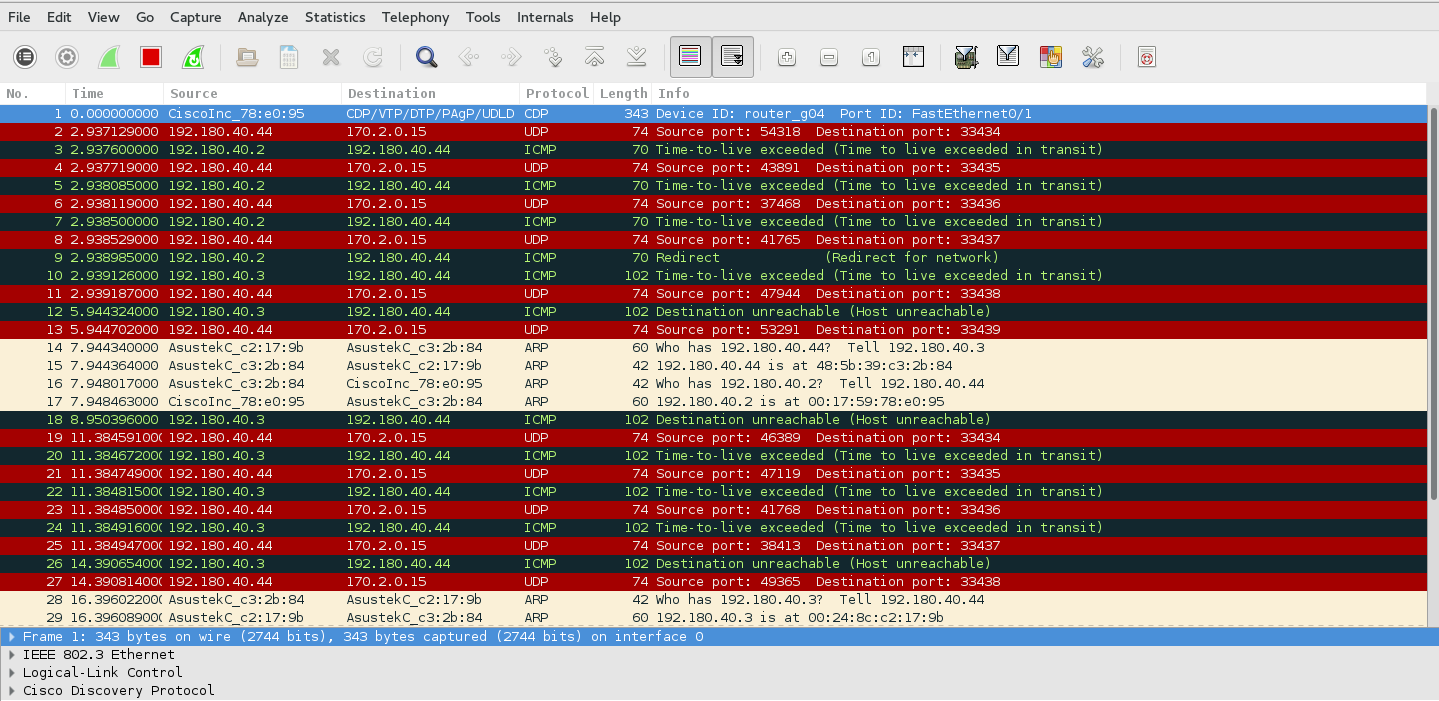
\includegraphics[width=0.9\textwidth, height=0.35\textheight]{1_g1_screenshot.png}
\label{fig:wireshark-enp0s7}
\caption{\emph{Screenshot} da captura de pacotes na interface enp0s7 (IP 192.180.40.44) no \emph{wireshark}.}
\end{figure}
\newpage
\subparagraph{ii)}
No capture do \emph{wireshark}, da figura anterior, podemos verificar que o \emph{router} Cisco envia um ICMP \emph{redirect message} para a máquina \textsf{Term2}, de modo a comunicar-lhe que existe uma melhor rota. Com esta informação o \textsf{Term2} atualiza a sua rota para o IP comunicado (192.180.40.3) e na chamada seguinte do \it{traceroute}, envia já diretamente para \textsf{RLin} (192.180.40.3), em vez de passar por \textsf{RCis2}, rota "antiga" (192.180.40.2).\\
O \emph{Internet Control Message Protocol}(ICMP) é usado, entre outras coisas, para os terminais e \emph{routers} trocarem informação sobre o seu funcionamento, controlo do fluxo de informação e para trocarem mensagens de controlo, bem como informação relativa à escolha de rotas até um determinado destino.\\
Um \emph{router} pode detetar uma rota alternativa entre o emissor e o recetor e enviar uma mensagem ao emissor, usando o ICMP, para o informar que existe uma melhor rota (ICMP \emph{redirect message}).